\section{Trajectory Planner}\label{CHAP: Method}

% \begin{itemize}
%     \item Tidligere kjent som 'Method'.
%     \item Har lyst å skrive litt om tankegangen bak utviklingen, ikke bare om hvordan ting endte opp med å bli.
%     \item Ingen 'Preliminaries', alt av forkunnskaper og antagelser burde vært gjort rede for i 'Background'.
%     \item Spesifikt mitt arbeid.
%     \item Tar det fra start til slutt. 
%     \subitem Persistent variables \& settings.
%     \subitem COLREGs assessment.
%     \subitem Dynamic Horizon.
%     \subitem Casadi setup (generer F)
%     \subitem Feasibility check.
%     \subitem Initial conditions and Reference LOS guidance.
%     \subitem NLP init.
%     \subitem Main loop, med alt som skjer der.
%     \subitem Solve NLP, give output.
%     \item Bit for bit, forklar hva, hvorfor, hvordan, eventuellt andre versjoner eller ideer som ble prøvd.
%     \item forklar informasjonsflyt, kanskje som eget delkapittel. 
%     \item My method is NOT a dock-to-dock system, the developed algorithm is NOT suitable for stationkeeping or docking maneuvers.
%     Dock-To-Dock does exist see \cite{WärtsiläDockToDock}, 
%     otherwise there are OTHER algorithms more suitable for docking. (TODO: FIND SOMETHING TO CITE)
% \end{itemize} 

% The developed algorithm is a path following trajectory planner and collision avoidance package where the dynamics of the \gls{OS}
% vessel are formulated as an ODE (TODO: REF TIL EQ) and the optimal trajectory is found by a method called direct multiple shooting.
% CasADi is employed to 

% The developed algorithm is a path following trajectory planner and collision avoidance package where the dynamics of the \gls{OS} vessel
% are modelled as ODEs and used together with a designed cost function to formulate an \gls{OCP}. The \gls{OCP} is solved numerically
% by transforming the problem into a \gls{NLP} with the help of a CasADi framework and a method called direct multiple shooting, 

% numerically
% through a direct multiple shooting method via a CasADi framework using an \gls{IPOPT} solver.


% (TODO: skriv bedre og mer korrekt.)
% This chapter presents the development of the trajectory planning and collision avoidance algorithm, explaining the design decisions made
% and analyzing some of the problems that arose during development. First the general dataflow of the algorithm is explained so that
% an intuition is formed as for how the individual parts are connected. Second a piece by piece construction of the algorithm up until
% the construction of the \gls{NLP}. Lastly the \gls{NLP} is constructed and solved using framework provided by CasADi. The core design
% of the algorithm is that path following is done through numerical optimization of a cost function, whilst collision avoidance and safety
% is implemented as hard constraints in the \gls{NLP}, together an optimal trajectory is formed. 

This chapter presents a step-by-step walkthrough of the developed trajectory planning and collision avoidance algorithm, and explains some of the
design decisions that were made during development. Additionally the chapter will include som analyzis of problems that arose during development,
and the implementationts that were made to overcome them. First the general dataflow of the algorithm is presented so that an intuition
can be gained as for how the individual parts of the algorithm are connected. Secondly each step of the algorithm is presented in the order of execution
from top to bottom. Lastly a brief look at how the output from the algorithm is put to use. 

The author wants to stress that while the trajectory planner is presented as a finished product, the algorithm was in active development until 12 days before
the thesis deadline. The code will have bugs, there will be unreadable spaghetti code, and at times logical errors. The code should have be delivered
as an attachment/appendix, or it can be found on github at: (TODO: LINK).

(TODO: enten i dette kapittelet eller i discussion må det skrives om tallverdi valg på funksjoner som dcpa grense etc.)
(TODO: bør vel også nevne at koden er skrevet i MATLAB? er ikke det mest brukte kodespråket i verden).

\subsection{Dataflow} (TODO: eller Overview?)
% \begin{itemize}
%     \item Begin by explaining the idea behind how the algorithm should work.
%     \item This chapter will need diagrams.
%     \subitem input $\rightarrow$ ??? $\rightarrow$ output
%     \subitem show how the internal functions parse data
%     \item Serves as a good overview of the whole algorithm.
% \end{itemize}
The core of the design is to construct a path following trajectory that is simultaneously able to comply with \gls{COLREGs} and avoid getting stuck
on terrain or other obstacles. The dataflow of the algorithm is depicted in Figure \ref{FIG: Dataflow chart}, 
to avoid clutter the diagram does not include every subfunction and minor detail, it's a
representative diagram, not a blueprint. On the left we begin with a higher level system, the algorithm
relies on getting information about it's own vessel and information about other ships, in the diagram called "tracks". Additionally
static obstacles and miscellaneous other settings for both debugging and behaviour tuning is to be supplied from said higher level system.

\begin{figure}[ht!]
    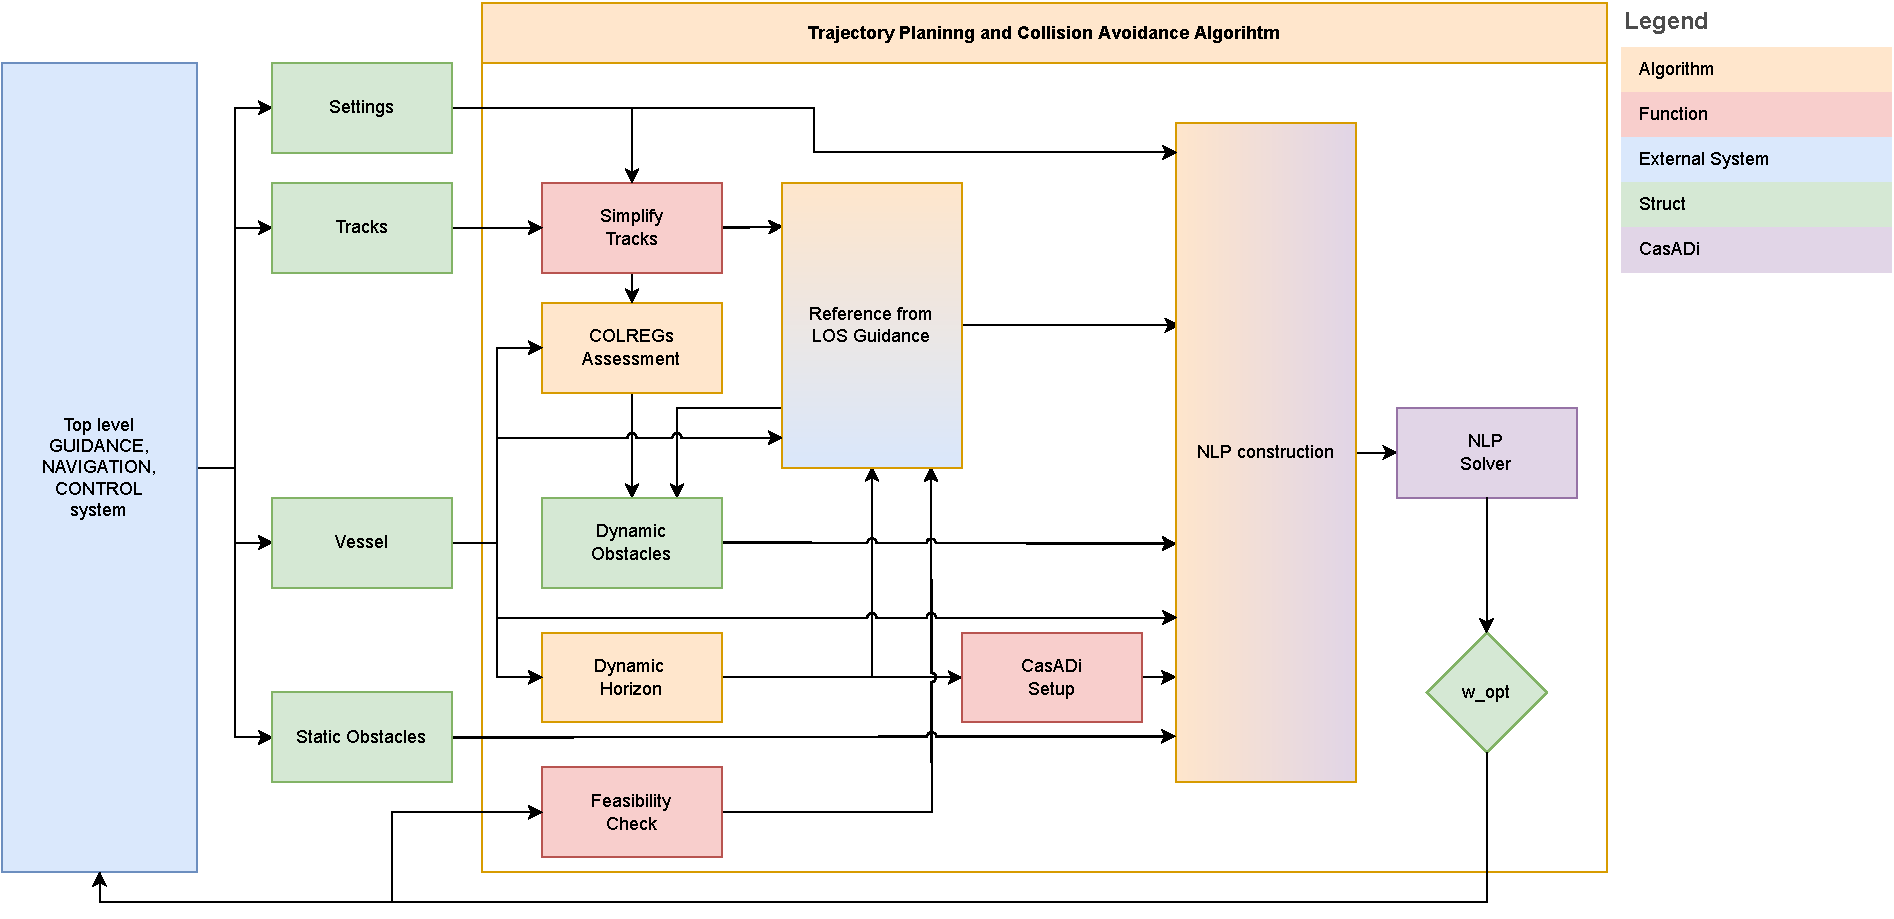
\includegraphics[width=\textwidth]{Images/SimpleSystem.pdf}
    \caption{A simplified overview of the developed algorithm.}
    \label{FIG: Dataflow chart}
\end{figure}

The algorithm is designed so that full prediction is the assumed standard prediction level. For testing and debugging purposes the tracks
structure can be modified to emulate the formfactor of a simple prediction level, in a real implementation the simplification should not be neccessary
as the data in the tracks struct should already be in the correct format for either prediction level.
The data in the tracks struct is parsed through a \gls{COLREGs} assessment algorithm to determine if any of the \gls{Ts}s need to be considered
an active dynamic obstacle. If a \gls{Ts} is deemed to be active the \gls{tCPA} and \gls{COLREGs} sitation is determined and kept as a flag. The flag
is stored in a persistent variable that the \gls{COLREGs} assessment algorithm checks to avoid overwriting the classification of an active situation.

Next, the information stored in the Vessel struct, the struct dedicated to the \gls{OS}, is used to calculate the desired time horizon for this call's
\gls{MPC}. Horizon distance and discretization step length are then needed by the CasADi setup function to create the \gls{RK4} method that
discretizes the vessel dynamics. On the very first call of the algorithm the feasibility check is skipped, because there is no previous trajctory to parse,
on all subsequent calls of the function the previously calculated optimal trajectory is checked for infeasibility. 
Feasibility, time horizon and discretization step information is then used to generate a reference trajectory for the \gls{OS}, a trajectory is
also generated for all the \gls{Ts} in the tracks struct, which are used to place dynamic constraints later.

The last step of the setup is to initialize the NLP using the \gls{OS}'s initial conditions, which creates the first
six decision variables of $\bm{\omega_0}$ and the first six elements of the constraint function $\textbf{g}(\bm{\omega})$.
Afterwars the algorithm iterates through all the control intervals, $NP$, from $K = 0:NP-1$, as decided by discretization step length and time horizon, 
constructing the NLP piece by piece in the following order:\newline
(TODO: Denne kan kanskje gjøres om til sånn fin algorithm type)\newline 
First three new decision variables $\bm{\tau_k}$ are made, the appropriate reference states are extracted from the reference trajectory, making sure
that the heading reference doesn't wrap the wrong way about $[0, 2\pi]$. Then the discretized dynamics are used to integrate one control interval
forward using $\bm{\omega_0}$, $\bm{\tau_k}$, and the reference values. Six new decision variables, $\bm{\omega_k+1}$, and their shooting
constraints are made. Lastly dynamic and static obstacles are placed in $\textbf{g}$ and k is incremented by one.

After the \gls{NLP} is constructed the initial guess for $\bm{\omega}$ is replaced by the previous optimal trajectory if it was feasible.
When the \gls{NLP} is solved the time it took is recorded, and if it didn't take too long to solve we save the solution to be used as the previous
optimal trajectory for the next time the algorithm runs. Some plots for debugging can then be made if desired, and the resulting optimal states
for the next control interval returned as the output of the algorithm.


\subsection{Setup}
% \begin{itemize}
%     \item All the stuff before main loop.
%     \item subsubsection for each 'block' as outlined by the dataflow.
% \end{itemize}

% \begin{itemize}
%     \item when the trajectory planner is called we need to run through some calculations before constructing the NLP problem
%     \item These calcualtions are a mix of situation analysis, simulation settings, and CasADi initialization.
%     \item Some of these calculations could be redundant in a complete control and navigation system,
%     where other modules of the system would calculate the same thing.
%     \item It's also important to remember that the value of many parameters are just guesswork, many of the subfunctions
%     would benefit from a more sophesticated design that are tuned based on the situation the vessel finds itself in.
% \end{itemize}
The setup is all of the code that is run from when the trajectory planning algorithm is called, up until the construction of the \gls{NLP}.
This is the modular part of the code, where functionality can easily be added or removed without having to refactor
the rest of the algorithm. Anything from new and improved situational awareness models to reference trajectory creation and
COLREGs compliance ideas slot right into the setup. Of course these mentioned systems could just as well exist outside of the
trajectory planning algorithm, but for this thesis it's designed as an all-in-one package.

In the current version of the trajectory planning algorithm there are four major and five minor tasks to get through
in the setup. First the major tasks:
\begin{itemize}
    \item Conduct COLREGs assessment.
    \item Calcualte dynamic horizon.
    \item Run CasADi initialization.
    \item Generate reference trajectories for \gls{OS} and \gls{Ts}s
\end{itemize}
and the 5 minor tasks:
\begin{itemize}
    \item Declare and initialize persistent variables.
    \item Initialize dynamic obstacles, and simplify tracks if needed.
    \item Conduct feasibility check on the previous optimal trajectory if it exists.
    \item Sanitize initial position to make sure there are no problems with the heading.
    \item fetch static obstacles, this is only a task because of how the MATLAB simulator is set up.
\end{itemize}

\subsubsection*{Persistent Variables} (TODO: vet ikke helt hvorfor jeg går så grundig til verks...)
In MATLAB, persistent variables are stored in memory when a script has terminated, and is loaded back as they were the next
time the script runs. This can be used to create rudimentary state machines, or to check the outcome of the previous iteration for anomalies.
Persistent variables are declared without an initialization, and the method for initializing them without overwriting every time is shown in Algorithm [\ref{ALG: PERSISTENT}].

\begin{algorithm}[h]
    \caption{Function: Initalize persistent variable} \label{ALG: PERSISTENT}
    \begin{algorithmic}
        \State \textbf{persistent} Var
        \If{isempty(Var)}
            \State Var $\gets$ Initial value
        \EndIf
    \end{algorithmic}
\end{algorithm}

Because persistent variables persist it is advised to manually clear the script when starting the MATLAB simulator, otherwise
residual perisstent variables from unrelated scenario files can cause debugging problems. In the algorithm there are seven
persistent variables. Two are used to store the optimal trajectory between iterations. One to store the discretized function F, so it doesn't have to be
remade every time the algorithm runs. one for storing COLREGs flag to act as a state machine. One for storing a variable called firsttime, 
used to execute code only the first time the algorithm is called. One that enables or disables obstacles, 
only left intact as a debugging tool. And the last one to store the previous iterations heading reference, which is used to prevent a
Wrap-to-2-Pi problem. (TODO: SKriv om hva Wrap-to-2-pi problem er for noe).

The reason there are two persistent variables to store the previous optimal trajectory is poor planning:
the original optimal trajectory was dumped if it took too long to solve the NLP. 
But later when I implemented a feasiblity check this would cause issues since feasiblity and time-to-solve for the NLP are not neccessarily linked.
Saving the previous optimal trajectory twice so that one is use for feasiblity check, while the other is the initial guess substitution candidate,
was a very quick hack solution that worked well enough that it survived until the final version of the code.


\subsubsection*{Simplify Prediction}
%Avansert TS prediction må skrives om i background.
%Tracks struct må forklares i background.
% This part of the setup is only required in simulations, the aim is to emulate the 'standard' way target ship (TS) prediction is conducted,
% which is to say constant course and velocity [TODO: Citation needed]. The TS trajectory is changed so that the first waypoint is the current position of the
% ship, and the next waypoint is one nautical mile in the direction of the ships heading. Ideally course over ground would be used instead of heading, however
% in the simulator crab angle and sideslip are not accounted for, therefor heading and course are the same angle.
% Excess waypoints stored in the TS struct are also truncated and the current waypoint index is forcefully set to 1 to prevent index out of range type errors.
This part of the setup is only neccessary in simulations, the idea is to prepare the tracks struct so that it can be parsed by the COLREGs assessment algorithm
regardless of desired prediction level. Since it is much easire to truncate excess waypoints and 'step down' from full prediction to simple, than the other way around, the algorithm
was developed with full prediction level as the standard. If it's desired to step down to a simple prediction level the tracks simply need to be parsed though algorithm [\ref{ALG: Simplify Tracks}].

% \begin{lstlisting}
%     for i = 1:size(tracks,2)
%         if simple
%             tracks(i).wp(1:2) = [tracks(i).eta(1);tracks(i).eta(2)];
%             tracks(i).wp(3:4) = [tracks(i).eta(1);tracks(i).eta(2)] +...
%                 1852 * [cos(tracks(i).eta(3)) , sin(tracks(i).eta(3))]';
%             tracks(i).wp = [tracks(i).wp(1:2)' tracks(i).wp(3:4)'];
%             tracks(i).current_wp = 1;
%         end
%         [dynamic_obs(i).cflag, dynamic_obs(i).dcpa, dynamic_obs(i).tcpa] = COLREGs_assessment(vessel,tracks(i),cflags(i));
%         cflags(i) = dynamic_obs(i).cflag;
%     end

% \end{lstlisting}
% (TODO: Bedre med algorithm eller MATLAB script insert?)
\begin{algorithm}[h]
    \caption{Function: Simplify \gls{Ts} prediction} \label{ALG: Simplify Tracks}
    \begin{algorithmic}
        \For{$i = 1:$size(tracks,2)}
            \If{simple}
                \State tracks($i$).wp(1:2) $\gets$ tracks($i$).eta(1:2)
                \State tracks($i$).wp(3:4) $\gets$ tracks($i$).eta(1:2) \\ \hfill + 1 nmi * [cos(tracks($i$).eta(3)) \ , \ sin(tracks($i$).eta(3))]\textsuperscript{T}
                \State tracks($i$).wp = [tracks($i$).wp(1:2)\textsuperscript{T} \ , \ tracks($i$).wp(3:4)\textsuperscript{T}]
                \State tracks($i$).current\_wp $\gets$ 1
            \EndIf
        \EndFor
    \end{algorithmic}
\end{algorithm}



\subsubsection*{COLREGs assessment}
% The COLREGs assessment function solves two problems; figuring out if\/when a TS vessel will be in close enough proximity that evasive maneuvers might be considered,
% and deciding which of the COLREGs rules will apply for the encounter. The design idea is to first find what the distance at closest point (dCPA) of approach with the TS is, and then
% time until cloest point of approach (tCPA) occurs. If both dCPA and tCPA values are under a set threshold we consider the encounter an active event and run the
% COLREGs situation assessment shown by \cite{Thyri2021b}. %COLREGs assessment is also explained in [TODO: fordypningsoppgaven].

% Finding the dCPA and tCPA between two vessels with constant velocity and course is easily done with a formula as shown by(eller in?) \cite{Kufoalor2018}.
%%%%%(TODO: SKRIV OM ALT DETTE, TING BLE FLYTTET HERFRA TIL KAPITTEL 2.3) %%%%%

%However with our wish for more advanced target ship prediction this formula is not sufficient on it's own.
%In order to achieve 'full coverage' of our intended path,
%nd the projected path of the target ship, we must check the dCPA and tCPA starting at each waypoint in the path of both vessels.
% helper function 'getCPAlist' is constructed to get the list of all dCPAs and their respective tCPAs when given two agent structs (AGENT STRUCTS MÅ FORKLARES I BACKGROUND) as inputs.
%o achieve full coverage the getCPAlist function is ran twice so that the perspective of each agent is considered. 

%In terms of code the function for COLREGs assessment uses the helper function getTCPAlist, which in turns uses three more helper functions. The first helper function vesselReadout
%returns the position and velocity in NED given a vessel struct and waypoint index as input. whereisTS gives the same output but takes an agent and time as input arguments instead.
%Lastly the function ClosestApproach takes the output from vesselReadout and whereisTS and applies the equations \eqref{eq:tCPAdCPA}. The dCPA, tCPA and positions are stored and the
%waypoint index is incremented by one, repeat until all waypoints 

% TODO: Ikke ferdig
% to get a list of all dCPA and tCPAs between two agents, as well as the corresponding positions of both
% agents as they are when the euqations \eqref{eq:tCPAdCPA} are used. getCPAlist 

% \begin{algorithm}[t]
%     \caption{getCPAlist. Denne ble jævelig stygg, beholder den for synlighet}\label{alg:getCPAlist}
%     \begin{algorithmic}[1]
%     \Require{$Agent1. Agent2$}\Comment{Agent is a struct that includes path waypoints}
%     \State $dCPAlist \gets []$
%     \State $tCPAlist \gets []$
%     \State $pos\_OS\_list \gets []$
%     \State $pos\_TS\_list \gets []$
%     \State $timer \gets 0$ \Comment{Initialize timer used to calculate position of Agent2}
%     \For{$i \gets Agent1.current\_wp : agent\_wplist\_length - 1$}
%         \State $[pos_{OS}, vel_{OS}] \gets VesselReadout(Agent1, i)$ \Comment{VesselReadout explained in algorithm...}
%         \State $DisttonextWP \gets $Distance to Agent1's next waypoint
%         \State $TimetonextWP \gets DisttonextWP \div$ Agent1's speed over ground
%         \State $[pos_{TS}, vel_{TS}] \gets whereisTS(Agent2, Timer)$ \Comment{whereisTS explained in algorithm...}
%         \State $[dCPA, tCPA] \gets$ Equation for dCPA \& tCPA as shown by...
%         \State $tCPA \gets tCPA + timer$ \Comment{Add travel time to reach current wp}
%         \State $timer \gets timer + TimetonextWP$
%         \State $pos\_OS\_list \gets [pos\_OS\_list, pos_{OS}]$ \Comment{Append all values to respective list.}
%         \State $pos\_TS\_list \gets [pos\_TS\_list, pos_{TS}]$
%         \State $dCPAlist \gets [dCPAlist, dCPA]$ 
%         \State $tCPAlist \gets [tCPAlist, tCPA]$ 
%         \State $i \gets i + 1$
%     \EndFor
%     \State \textbf{return} $pos\_OS\_list, pos\_TS\_list, dCPAlist, tCPAlist$
%     \end{algorithmic}
% \end{algorithm}

(TODO: synes dette kapittelet er elendig beskrevet, vet ikke om jeg orker skrive det bedre).

The COLREGs assessment algorithm solves two problems, the first is figuring out if a \gls{Ts} vessel will be be within close enough proximity that it should be considered
an active COLREGs situation. The second problem is deciding which COLREGs situation such a encounter might be. For two vessels with constant speed and course this is a rather
simple task; first apply the equations \eqref{eq:tCPAdCPA}, and then run a COLREGs assessment function such as one laid out by (\cite{Thyri2021b}). However if we want
to take advantage of full prediction level a bit more logic is needed to assure full coverage of the intended path. Another functionality needed to ensure COLREGs compliance
is a state machine that holds onto the designated COLREGs situations, the rules state that once a situation has started it persists until both vessels are clear of each other.

The idea for the implementation in this thesis is to extend the \gls{dCPA} and \gls{tCPA} check so that it's conducted for every waypoint in the \gls{OS} and \gls{Ts} reference path.
That way it's possible to know roughly where both vessels should be at the \gls{dCPA} point. The COLREGs assessment
algorithm is therefor split into two parts; the first part is an extended CPA check, the second part is the COLREGs situation assessment. 

A function getCPAlist is created to take two vessel structs as input, one as the assigned \gls{OS}, and the other the \gls{Ts}. The function iterates through all the waypoints
in the \gls{OS} assigned struct and does three things:\newline
Figure out the pose of the \gls{OS} and \gls{Ts}.\newline
Run the CPA check from said pose.\newline
Calculate the time and distance to next \gls{OS} waypoint so that the pose of the \gls{Ts} at that point can be accurately found.

Finding the pose of the \gls{OS} is trivial, the first iteration of the function the pose is just the current positon and course of the vessel, for all
subsequent waypoints the waypoints themselves are the position and the heading is the direction towards the next waypoint. The last waypoint does not need to be checked
because at that point the \gls{OS} stops moving. While this is a fantastically simple way of interating forward through the waypoints, the tradeoff is less accuracy of the CPA check
when turning. 
Finding the pose of the \gls{Ts} is slightly more involved, since there are no waypoints to lean on the method here is different than for the \gls{OS}.
To begin we know where the \gls{Ts} is when the check is conducted, time and an assumption of constant velocity is then used to calculate the pose.
(TODO: hvordan vise dette uten å ta med hele kodesnutten?).
% \begin{lstlisting}
%     function [pos_TS, vel_TS] = whereisTS(tracks,wptstimer)
%     pos_TS = tracks.eta(1:2);
%     vel_TS = tracks.eta_dot(1:2);
%     WPlim = size(tracks.wp,2);

%     pos = tracks.eta(1:2);
%     distance = wptstimer * norm(tracks.nu(1:2),2);
%     WPindex = tracks.current_wp;
%     if WPindex < WPlim
%         distancetonextWP = sqrt((tracks.wp(1,WPindex+1) - pos(1))^2 + ((tracks.wp(2,WPindex+1) - pos(2))^2));
%     else
%         distancetonextWP = 0;
%     end
%     while distance > 0
%         if distance > distancetonextWP
%             pos = tracks.wp(1:2,WPindex+1);
%             distance = distance - distancetonextWP;
%             WPindex = WPindex + 1;
%             if WPindex < WPlim
%                 distancetonextWP = sqrt((tracks.wp(1,WPindex+1) - pos(1))^2 + ((tracks.wp(2,WPindex+1) - pos(2))^2));
%             else
%                 distancetonextWP = 0;
%                 pos_TS = pos;
%                 vel_TS = [0,0]';
%                 distance = 0;
%             end
%         else
%             direction = tracks.wp(:,WPindex+1) - pos;
%             travel = distance / distancetonextWP;
%             pos_TS = pos + travel * direction;
%             vel_TS = rotZ(atan2(direction(2),direction(1))) * tracks.nu;
%             vel_TS = vel_TS(1:2);
%             distance = 0;
%         end
%     end
% end    

% \end{lstlisting}
% Here, wptstimer is calculated as the time it would have taken the \gls{OS} to reach the current active waypoint. 
With the pose of both vessels calculated, the next step is to check the CPA, which is the same equation as \eqref{eq:tCPAdCPA}, the values for
\gls{dCPA} and \gls{tCPA}, as well as the pose of both vessels are stored in vectors for later. The \gls{tCPA} value is also added to a timer which is
used to track how much time is passing for the \gls{OS} to reach the checked waypoints.
The full path CPA check is then ran with the vessel inputs flipped, so that the \gls{Ts} waypoints are checked, the lowest values of each CPA list
are then compared to select which \gls{dCPA} is truly the shortest distance. If both dCPA and tCPA are under some set threshold a COLREGs classification is set.
(TODO: [...] as described? det er jo referert til tre forskjellige kilder med metoder, tror det skal være greit forstått).

\subsubsection*{Dynamic Horizon}
% \begin{itemize}
%     \item Dynamic horizon is a balancing act between distance to goal, encompassing all active dynamic obstacles, and not looking to far ahead into the future.
%     \item changing the dynamic horizon is really just changing how many control intervals we want the NLP to have.
%     \item As the distance to goal approaches zero we want the number of control intervals to shrink accordingly, otherwise we end up with too many control intervals stationary at the goal, which can cause problems like the cost function becoming unbalanced.
%     \item If there are active dynamic obstacles we need the dynamic horizon to encompass them.
%     \item we don't want the dynamic horizon to be too short during transit (why not?).
% \end{itemize}
The purpose of the dynamic horizon is to shorten the amount of control intervals when the \gls{OS} approaches the final destination. The reason for this
is that having many control intervals stationary at the end position can unbalance the cost function and lead to poor performance for the remainder of the path.
The dynamic horizon can also be coded so that it's dynamic with respects to COLREGs situations; always having enough control intervals to clear the furthet out
COLREGs situation, but less control intervals than the nominal value so the \gls{NLP} can be solved faster, which would lead to a better reactive performance.

The distance between two waypoints $\textrm{WP}_1 = (N_1, E_1)$,  $\textrm{WP}_0 = (N_0, E_0)$  is calculated with by the following equation:
\begin{equation}
    D_{1} = \sqrt{(N_1 - N_0)^2 + (E_1 - E_0)^2}
\end{equation}
which means the distance to goal is the sum of all distances between waypoints:
\begin{equation}
    D_{goal} = \sum_{\textrm{wp} = 1}^{N} D_{wp}
\end{equation}
with $\textrm{WP}_0$ being the position of the \gls{OS} and $\textrm{WP}_N$ being the goal. Assuming a near constant velocity the time to
reach goal is:
\begin{equation}
    T_{goal} = \frac{D_{goal}}{u}
\end{equation}
where $u$ is the surge of the \gls{OS}. It's not neccessary for this check to be 100\% accurate, it is expected that the \gls{OS} will deviate from the
path due to physical constraints and obstacles anyway.


\subsubsection*{CasADi setup}
% \begin{itemize}
%     \item sym x = [N, E, psi, u, v, r]
%     \item sym tau as a free variable
%     \item sym xref as reference
%     \item model parameters
%     \item M, C, D matrix
%     \item xdot \= [nu\_dot, eta\_dot]
%     \item Error in the correct reference frame.
%     \item Why is the cost function the way it is.
%     \item runge-kutta method.
%     \item the final function F that CasADi needs.
%     \item Noe av disse greiene blir dekt av Background, forhåpentligvis.
% \end{itemize}

\subsubsection*{Feasibility check}
% \begin{itemize}
%     \item The feasibility check came from the wish to read out the status report CasADi prints to the command window.
%     \item It's very important to know if the previous iteration of the trajectory planner function yielded a feasible result or not.
%     \item if the result is not feasible the path forward might be completely blocked, in which case reducing our vessel speed is the best option.
%     \item Very simple check, just checks if every point in the previously calculated optimal trajectory is within 5 meters of each other. This is very lenient and should of course change depending on vessel speed.
% \end{itemize}

\subsubsection*{Reference from LOS}
% \begin{itemize}
%     \item I didn't write this \:)
%     \item The important part is that the time discretization is consistent with the trajectory planner's time step
%     \item You don't need to use LOS for reference.
%     \item Position reference and speed reference need to be consitent with each other.
% \end{itemize} 


\subsection{NLP Construction and Solver} 
% \begin{itemize}
%     \item inputs\: vessel, ref\_trajectory, static\_obs, dynamic\_obs, F, settings, h, N, previous\_w\_opt.
%     \item sub funksjoner\:
%     \subitem Dynamic Obs.
%     \subitem Static Obs.
%     \subitem integration step.
%     \item output\: w\_opt
% \end{itemize}

\subsubsection{NLP initialization}
% \begin{itemize}
%     \item Initial conditions and end of interval coditions, we need the end of one control interval and the beginning of the next to match.
%     \item Tror dette delkapittelet er litt unødvendig
% \end{itemize}

\subsubsection{Integration step}
% \begin{itemize}
%     \item Getting the correct reference
%     \item make sure all the indexes are correct!
%     \item put the references in w0, speeds up runtime significantly.
% \end{itemize}

\subsubsection{Dynamic Obstacles constraints}
% \begin{itemize}
%     \item When to place constraints
%     \item Where to place them
%     \item How to place them
% \end{itemize}

\subsubsection{Static Obstacles constraints}
% \begin{itemize}
%     \item Explain static\_obstacles\_check and the theory for convex-free set
%     \item explain why circles, such as the ones used for dynamic obstacles are insufficient.
%     \item this is sort of similar to finding a cross track error, if that helps to explain what is going on.
% \end{itemize}

\begin{figure}[ht]
    \centering
    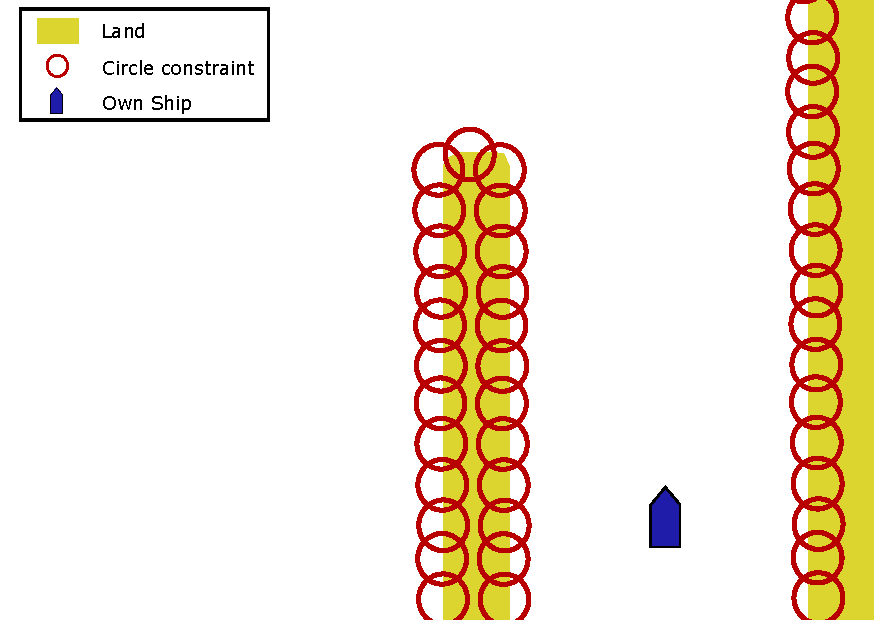
\includegraphics[width=\textwidth]{Images/StaticObs_Naive.pdf}
    \caption{TODO: SKRIV OG REFERER. Naiv approach 1}     \label{FIG: Static Obs Naive approach 1}
\end{figure}

\begin{figure}[ht]
    \centering 
    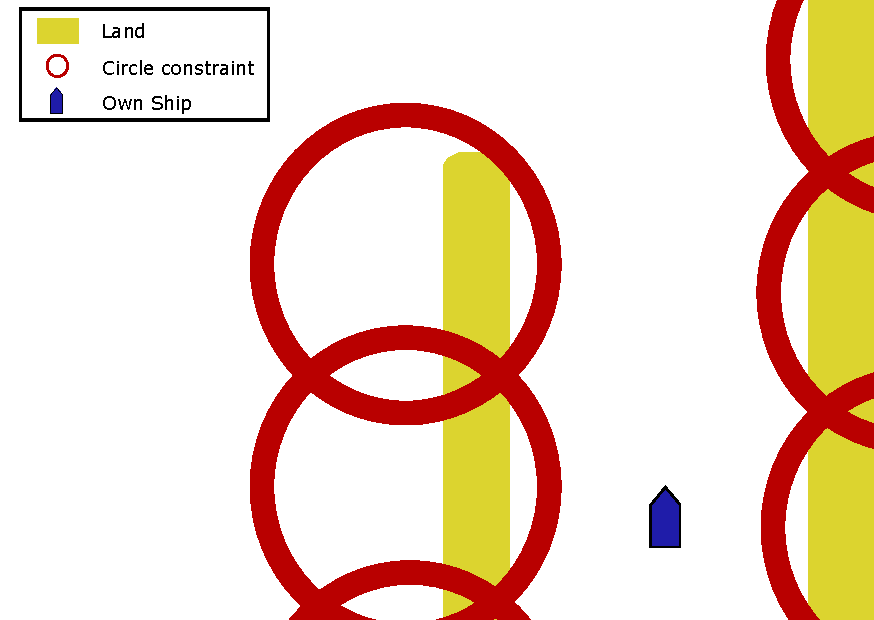
\includegraphics[width=\textwidth]{Images/StaticObs_Naive2.pdf}
    \caption{TODO: SKRIV OG REFERER. Naiv approach 2}     \label{FIG: Static Obs Naive approach 2}
\end{figure}

\begin{figure}[ht]
    \centering
    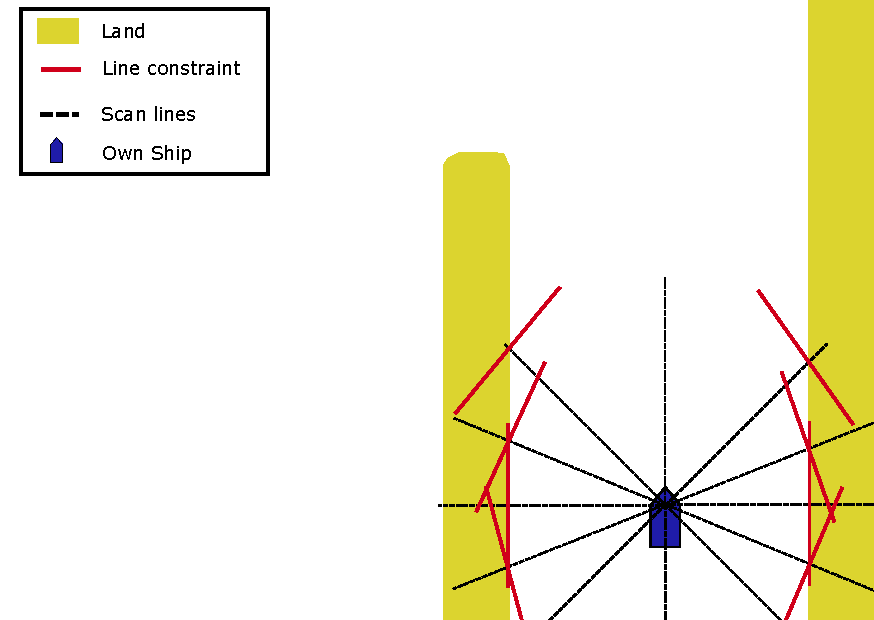
\includegraphics[width=\textwidth]{Images/StaticObs_lines.pdf}
    \caption{TODO: SKRIV OG REFERER. Convex free set}     \label{FIG: Static Obs Lines}
\end{figure} 

\subsubsection{Solver}
% \begin{itemize}
%     \item Options, there are many options.
%     \item things to try / were tried for optimizing runtime.
%     \item CasADi really does all the hard work.
% \end{itemize}

% \subsection{Alternative Ideas and Lessons}
% Burde kanskje heller gå under discussion, og igjen i future work.
% \begin{itemize}
%     \item Change w0 based on previous solution runtime.
%     \item Gamle versioner av Static\_obs.
%     \item eksperimenter med feasibility check.
%     \item Masse styr med COLREGs assessment, tcpa og dcpa.
%     \item ipopt innstillinger.
% \end{itemize}

\newpage